\chapter[Proposta Metodológica]{Proposta Metodológica}
Este capítulo apresenta os procedimentos e métodos a serem utilizados para desenvolvimento deste presente
 trabalho, detalhando as metodologias \textit{Bottom-Up}, utilizadas nas implementações tanto em hardware
 quanto em software, além das linguagens de programação utilizadas nas implementações e suas respectivas
 ferramentas. Por fim é apresentado um cronograma de atividades.

\section{Implementação em hardware}
Esta seção apresenta os dispositivos e ferramentas a serem utilizados neste presente trabalho, além das metodologias a serem desenvolvidas, para implementação do algoritmo de treinamento do classificador LDA em Hardware.

\subsection{Dispositivos e ferramentas}
Visando as grandes vantagens de utilização dos SoCs, o algoritmo de treinamento do classificador
 LDA será implementado nas lógicas digitais da FPGA na plataforma Zynq da placa \textit{Zybo-Board}, utilizando
 os \textit{IP-Cores}, que são blocos matemáticos desenvolvidos com propriedades intelectuais \cite{munoz2010tradeoff} em unidade de ponto flutuante desenvolvidos por \cite{munoz2010tradeoff} e a linguagem de programação \textit{VHSIC Hardware Description Language} (VHDL), a fim de paralelizar os
 processos do algoritmo. Para o mapeamento do algoritmo em VHDL será utilizado a plataforma 
\textit{Vivado HLS}, que possui todas as ferramentas necessárias para descrição, simulação, implementação e mapeamento hardware que descreve o algoritmo na FPGA \cite{zynqBook}.

\subsection{Metodologias de desenvolvimento}
Para desenvolvimento do algoritmo será adotada a metodologia \textit{bottom-up}, onde cada sub-bloco desenvolvido é testado antes de ser inserido ao bloco principal, bloco de integração de todos sub-blocos do projeto, também conhecido como \textit{Top module}.
Após a implementação e simulação do \textit{Top module}, será utilizado para teste e validação do hardware
 o \textit{dataset IVa} do \textit{BCI Competition III}, além de uma análise estatística do erro apresentado
 quando comparado com o desenvolvimento na plataforma \textit{Matlab} por \cite{F.Lotte}.

Para validação da eficiência do SoC serão coletados os dados das seguintes características:
\begin{itemize}
	\item Consumo de hardware: LUTs, FFs, blocos de DSP, blocos de memória RAM, I/O, MUX;
	\item Dados de desempenho: frequência de operação e tempo de execução;
	\item Estimação do consumo de potência.
\end{itemize}

Os processos de implementação do hardware em um SoC é apresentado na Figura \ref{diagram_hardware}.

\begin{figure}[h]
	\centering
	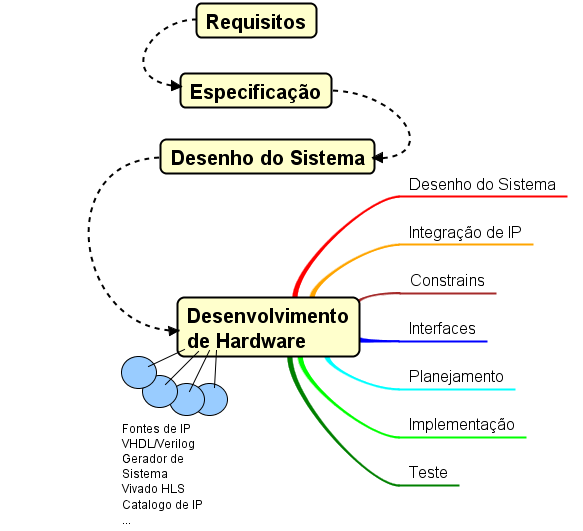
\includegraphics[keepaspectratio=true,scale=1.0]{figuras/fluxograma_hardware.PNG}
	\caption{Fluxograma de implementação de hardware em um SoC. Adaptado de \cite{zynqBook}}
	\label{diagram_hardware}
\end{figure}

\section{Implementação em software}
São apresentados nesta seção, os materiais, métodos e técnicas para a implementação do
algoritmo de treinamento do classificador LDA em software.

\subsection{Materiais}

Dispondo do SoC embarcado no kit de desenvolvimento da Digilent(\textit{Zybo-Board}) , a implementação do algoritmo em 
software, explorará o processador \textit{ARM$^{\textregistered}$  Cortex$^{\textregistered}$ -A9} de dois núcleos no \textit{Xilinx Zynq$^{\textregistered}$ -7000}, usando também
o auxílido do sistema operacional xilinux, a codificação do algorítmo será feita dipondo das linguagens de programação
C e C++.

\subsection{Métodos e Técnicas}
 
Para o auxílio desta implemetação, será instalado o sistema operacional \textit{Xilinux}, os recursos e passos necessários
para a instalação do S.O estão contidos no \cite{zynqBook}.
O processo para implementação seguirá o método \textit{bottom-up}, blocos de códigos menores serão implementados e testados
separadamente, com a finalização de todos os blocos finalmente será integrado e testado por completo, as entradas
para programa desenvolvido são provinientes do \textit{dataset IVa} do \textit{BCI Competition III}.

 
Os dados para análise pós implementação e teste serão:
\begin{itemize}[noitemsep]
\item Consumo de memória
\item Tempo de execução
\item Consumo de potência
\item Erro da implementação em comparação com os resultados obtidos por \cite{F.Lotte}
\end{itemize}













\section{\textit{Data Set IVa}}

Em ambas as implementações serão utilizadas o \textit{Data Set IVa} da \textit{BCI Competition III} \cite{BCICompetition}, para efeito de testes e validações do sistema.
Os dados \textit{Data Set IVa} foram adquiridos e armazenados utilizando amplificadores do tipo \textit{BrainAmp} e uma capa de eletrodos de 128 canais. Foram utilizados 118 canais de EEG posicionados de acordo com o sistema 10/20. Cada um destes canais foram filtrados em banda passante, utilizando um filtro \textit{butterworth} de quinta ordem entre as frequências de 0.05 e 200 Hz, posteriormente foram digitalizados com uma frequência de amostragem de 1 kHz com precisão de 16 bits, apresentando uma resolução de 0.1 $\mu$V, além disso também foram disponibilizados os mesmos dados com uma frequência de amostragem de 100 Hz \cite{siteBCI}.


\section{Cronograma de Atividades}
Esta seção apresenta o cronograma de desenvolvimento deste presente trabalho.

As atividades já desenvolvidas são apresentadas no cornograma da tabela \ref{conograma1}
As atividades a serem desenvolvidas por cada um dos autores é apresentada no cronograma da Tabela \ref{cronograma2}, onde as atividades atribuídas ao autor Heleno da Silva Morais são referenciada simbolicamente com a letra "X" enquanto as atividades atribuídas ao autor Oziel da Silva Santos são referenciadas simbolicamente pela letra "O".

\begin{table}[]
	\centering
	\caption{Cronograma de atividades já desenvolvidas para este presente trabalho}
	\label{cronograma1}
	\begin{tabular}{|l|c|c|c|c|c|}
		\hline
		\textbf{Atividade} & \multicolumn{1}{l|}{\textbf{Agosto}} & \multicolumn{1}{l|}{\textbf{Setembro}} & \multicolumn{1}{l|}{\textbf{Outubro}} & \multicolumn{1}{l|}{\textbf{Novembro}} & \multicolumn{1}{l|}{\textbf{Dezembro}} \\ \hline
		\textit{\begin{tabular}[c]{@{}l@{}}Pesquisa\\ Bibliográfica\end{tabular}} & XO & XO & XO & XO & XO \\ \hline
		\textit{Escolha do Tema} & XO & XO &  &  &  \\ \hline
		\textit{\begin{tabular}[c]{@{}l@{}}Pesquisa da Base\\ de Dados\end{tabular}} & XO & XO & XO &  &  \\ \hline
		\textit{\begin{tabular}[c]{@{}l@{}}Pesquisa de Algoritmos\\ já Desenvolvidos\end{tabular}} &  & XO & XO & XO &  \\ \hline
		\textit{\begin{tabular}[c]{@{}l@{}}Análise do Algoritmo\\ Desenvolvido \\ por\cite{F.Lotte}\end{tabular}} &  &  &  & XO & XO \\ \hline
		\textit{\begin{tabular}[c]{@{}l@{}}Reprodução dos\\ Resultados obtidos por\\ \cite{F.Lotte}\end{tabular}} &  &  &  & XO & XO \\ \hline
		\textit{\begin{tabular}[c]{@{}l@{}}Documentação do\\ Projeto\end{tabular}} &  &  & XO & XO & XO \\ \hline
		\textit{Apresentação do Projeto} &  &  &  &  & XO \\ \hline
	\end{tabular}
\end{table}


\begin{table}[]
	\centering
	\caption{Cronograma de atividades a serem desenvolvidas para este presente trabalaho.}
	\label{cronograma2}
	\begin{tabular}{|l|c|c|c|c|c|c|}
		\hline
		\textbf{Atividade} & \multicolumn{1}{l|}{\textbf{Fevereiro}} & \multicolumn{1}{l|}{\textbf{Março}} & \multicolumn{1}{l|}{\textbf{Abril}} & \multicolumn{1}{l|}{\textbf{Maio}} & \multicolumn{1}{l|}{\textbf{Junho}} & \textbf{Julho} \\ \hline
		\textit{\begin{tabular}[c]{@{}l@{}}Pesquisa\\ Bibliográfica\end{tabular}} & XO & XO & XO & XO & XO & XO \\ \hline
		\textit{\begin{tabular}[c]{@{}l@{}}Implementação do \\ Algoritmo em FPGA\end{tabular}} & X & X & X & X &  &  \\ \hline
		\textit{\begin{tabular}[c]{@{}l@{}}Teste da Implementação\\ em FPGA\end{tabular}} & X & X & X & X & X &  \\ \hline
		\textit{\begin{tabular}[c]{@{}l@{}}Validação da\\ Implementação em FPGA\end{tabular}} &  &  &  &  & X & X \\ \hline
		\textit{\begin{tabular}[c]{@{}l@{}}Levantamento das\\ Características descritas\\ na seção 3.1.2\end{tabular}} &  &  &  &  & X & X \\ \hline
		\textit{\begin{tabular}[c]{@{}l@{}}Análise Estatística do \\ Erro Obtido com a\\ Implementação em FPGA\end{tabular}} &  &  &  &  & X & X \\ \hline
		\textit{\begin{tabular}[c]{@{}l@{}}Instalação do SO\\ Xilinux nos Core ARM\end{tabular}} & O & O &  &  &  &  \\ \hline
		\textit{\begin{tabular}[c]{@{}l@{}}Implementação do\\ Algortimo em Software\\ Embarcado\end{tabular}} &  & O & O & O &  &  \\ \hline
		\textit{\begin{tabular}[c]{@{}l@{}}Testes do Algoritmo\\ Implementado em\\ Software Embarcado\end{tabular}} & O & O & O & O & O &  \\ \hline
		\textit{\begin{tabular}[c]{@{}l@{}}Validação da \\ Implementação em\\ Software Embarcado\end{tabular}} &  &  &  &  & O & O \\ \hline
		\textit{\begin{tabular}[c]{@{}l@{}}Análise Estatística do\\ Erro Obtido com a \\ Implementação em \\ Software Embarcado\end{tabular}} &  &  &  &  & O & O \\ \hline
		\textit{Documentação do Projeto} & XO & XO & XO & XO & XO & XO \\ \hline
		\textit{Apresentação do Projeto} &  &  &  &  &  & XO \\ \hline
	\end{tabular}
\end{table}
